\documentclass[a4paper,10pt,titlepage]{article}

\usepackage{geometry}
\usepackage{amsmath}
\usepackage{amssymb}
\usepackage{txfonts}
\usepackage{microtype}
\usepackage{epsfig}
\usepackage{graphicx}
\usepackage{moreverb}
\usepackage{hyperref}
\usepackage{listings}
\usepackage{xcolor}
\usepackage{textcomp}
\definecolor{listinggray}{gray}{0.98}
\definecolor{lbcolor}{rgb}{0.98,0.98,0.98}
\lstset{
	backgroundcolor=\color{lbcolor},
	tabsize=4,
	rulecolor=,
	language=matlab,
    basicstyle=\scriptsize\ttfamily,
    upquote=true,
    aboveskip={1.5\baselineskip},
    columns=fixed,
    showstringspaces=false,
    extendedchars=true,
    breaklines=true,
    prebreak = \raisebox{0ex}[0ex][0ex]{\ensuremath{\hookleftarrow}},
    frame=single,
    showtabs=false,
    showspaces=false,
    showstringspaces=false,
    identifierstyle=\ttfamily,
    keywordstyle=\color[rgb]{0,0,1},
    commentstyle=\color[rgb]{0.133,0.545,0.133},
    stringstyle=\color[rgb]{0.627,0.126,0.941},
}
\usepackage{eso-pic}
\usepackage{ifthen}

\AddToShipoutPictureBG{\ifthenelse{\equal{\value{page}}{0}}{}{
\includegraphics{template_files/backgroundlines}}}

\usepackage{units}
%\usepackage[T1]{fontenc}
%\usepackage[utf8]{inputenc}
\usepackage{physics}

\newcommand{\ee}{\mathrm{e}}
\newcommand{\ii}{\mathrm{i}}

\title{H1b: MD simulation -- dynamic properties}
\author{Andr\'eas Sundstr\"om and Linnea Hesslow}
\date{\today}

\begin{document}

\newgeometry{top=2cm,bottom=2cm,left=2cm,right=2cm}

\begin{titlepage}

\setcounter{page}{0}

\begin{center}
{\huge \bf \color{red} NB: The graded, first version of the report must be
                           returned if you hand in a second time! } \\
\vspace{3cm}
\makeatletter
{ \huge \@title } \\
\vspace{1cm}
{ \Large \@author }\\
\vspace{1cm}
{ \Large \@date }\\
\makeatother
\end{center}

\vfill

\begin{flushright}
{\Large
\begin{tabular}{|c|c|c|}
\hline
Task N\textsuperscript{\underline{o}} & Points & Avail.\ points \\ \hline
\hspace{3cm} & \hspace{3cm} & \hspace{3cm} \\ \hline
~ & ~ & ~ \\ \hline
~ & ~ & ~ \\ \hline
~ & ~ & ~ \\ \hline
~ & ~ & ~ \\ \hline
~ & ~ & ~ \\ \hline
~ & ~ & ~ \\ \hline
~ & ~ & ~ \\ \hline
$\sum$ & ~ & ~ \\
\hline
\end{tabular}}
\end{flushright}

\end{titlepage}

\newgeometry{top=2cm,bottom=2cm,left=1.5cm,right=7.4cm}


\section*{Introduction}

.... TODO... !!!!!!!!!!!!!!!!!!!!!

\section*{Task 1: potential energy}
The theoretical lattice parameter for aluminim can be determined by calculating the minimum potential energy per unit cell in a lattice with zero initial momenta for all particles. 

Figure~\ref{fig1} shows the potential energy as a function of the lattice parameter. We used a quadratic fit to find the minimum energy, and obtained $V_{\rm eq} \approx \unit[65.38]{\AA^3}$. This corresponds to the equilibrium lattice parameter $a_{\rm eq} \approx \unit[4.029]{\AA}$ at \unit[0]{K}, which we took as the initial lattice parameter for the following tasks.  

\begin{figure}[!ht]
\begin{center}
  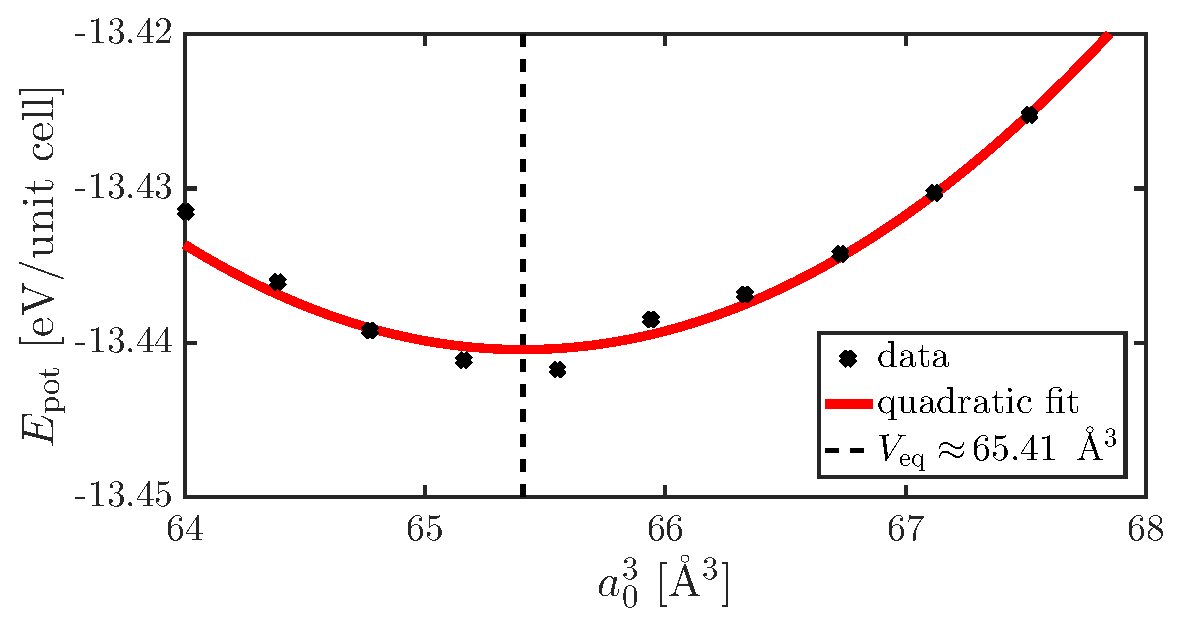
\includegraphics[width=0.7\textwidth]{../figures/potential_energy} 
  \caption{The potential energy per unit cell for aluminum as a function of the lattice parameter cubed.}
  \label{fig1}
\end{center}
\end{figure}

We find that figure~\ref{fig1} looks similar to the figure~1 in the homework problem file. 

%%%%%%%%%%%%%%%%%%%%%%%%%%%%%%%%%%%%%%%%%%%%%%%%%%%%%%%
\section*{Task 2: detmine the timestep}


With the random noise, the temperature and the energy are differs between runs, but are in the same order of magnitude. From figure~\ref{fig:task2}, we determine that $dt = \unit[5 \cdot 10^{-3}]{ps} = \unit[5]{fs}$ is a sufficient time step. This is in line with the lecture notes, where it is stated that the a suitable timestep would normally be a few femtoseconds, or somewhat larger for heavy atoms.
  
We note that the temperature is higher than desired value of~\unit[600-800]{K}. The temperatures and energies up to one standard deviation are quantified in table~\ref{tab:task2}. 



\begin{figure}[!ht]
\begin{center}
  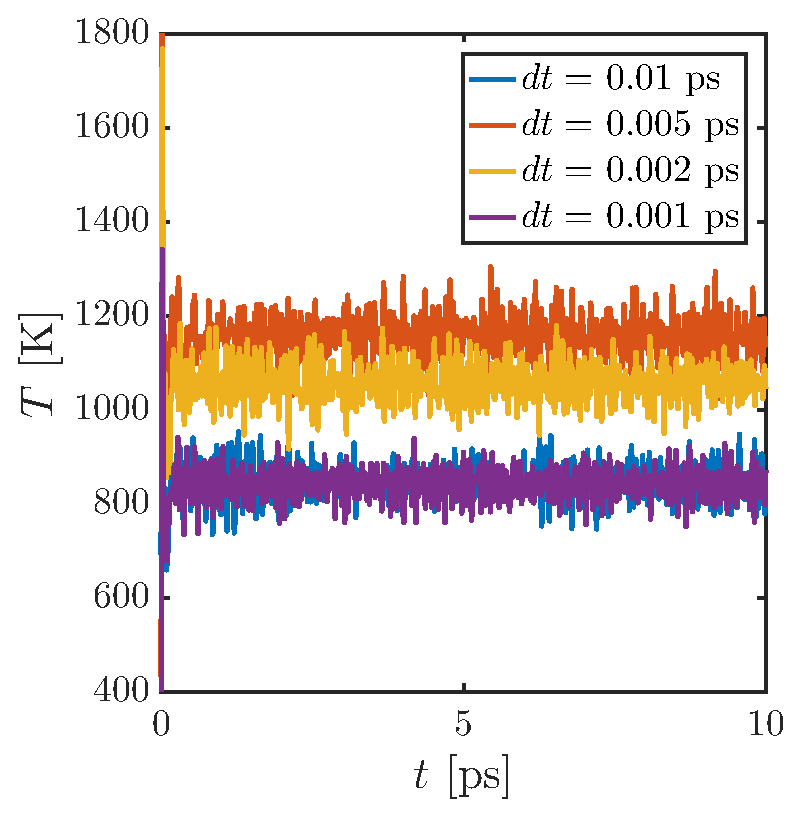
\includegraphics[width=0.48\textwidth]{../figures/dt-scan-temperature} 
    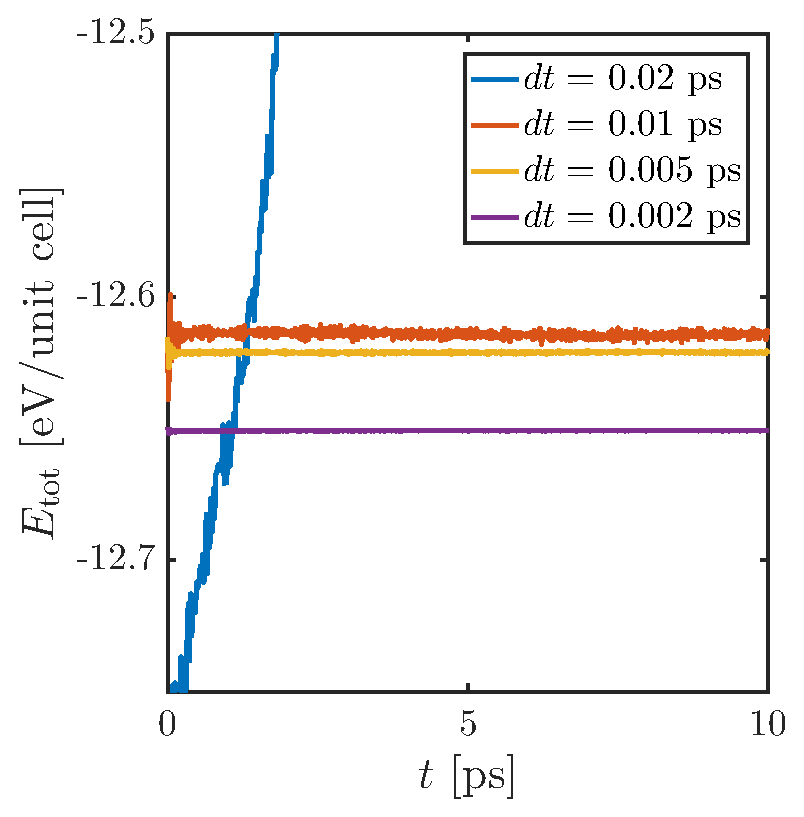
\includegraphics[width=0.48\textwidth]{../figures/dt-scan-energy} 
  \caption{The temperature and kinetic energy per unit cell as a function of time for four different timesteps.}
  \label{fig:task2}
\end{center}
\end{figure}



\begin{table}[!ht]
  \begin{center}
    \caption{Energies and temperatures with one standard deviation uncertainties for four different values of the time steps.}
    \begin{tabular}{l c c} 
    $dt$ [ps] & $T$ [K] & $E_{\rm tot}$ [eV/unit cell]\\ \hline
$10^{-2}$ & 	$847 \pm 4.2\%$ &	$-12.55 \pm 1.2\cdot 10^{-2} \% $\\
$5\cdot 10^{-3}$ &	$1157 \pm$ 3.8 \% &$-12.24 \pm 3.6\cdot 10^{-3} \%$ \\
$2\cdot 10^{-3}$ & $1058  \pm 3.7 \% $ & 	$ -12.35 \pm 6.6\cdot 10^{-4} \% $\\ 
$1\cdot 10^{-3}$ & $ 841  \pm 3.7 \% $	 &$ -12.58 \pm 3.6\cdot 10^{-4} \%$ \\ 
      \hline
    \end{tabular}
    \label{tab:task2}
  \end{center}
\end{table}

\section*{Tasks 3 and 4: Temperature and pressure equilibration}
We set $\tau_P = \tau_T = 100 dt$, where $dt = 5\cdot 10^{-3}$\,ps, and equilibrated the temperature and pressure by scaling the particle momenta and positions (and box size) respectively. Choosing a slower equilibration time did not affect the results qualitatively. Both temperature and pressure were equilibrated in the same Verlet loop, but for the higher temperature the the system was first melted by increasing the temperature to \unit[900]{$^\circ$C}. To determine the isothermal compressibility $\kappa$, 
the values of Young's modulus $Y$ and shear modulus $G$ were taken from Physics Handbook, table T 1.1. From F 1.15 in Physics Handbook, the bulk modulus can then calculated as
\begin{equation}
B = \frac{YG}{9G - 3Y} \,\quad \kappa_{\rm Al} = \frac{1}{B} \approx \unit[6.6444\cdot 10^5]{bar},
\end{equation}
where \unit[1]{bar } = $\unit[6.2415\cdot 10^{-7}]{eV/\AA^3}$ in atomic units. \textbf{However, we set $\kappa = 100 \kappa_{\rm Al}$ since the pressure equilibration happened on a much longer timescale than $\tau_P$ with $\kappa = \kappa_{\rm Al}$. We have not yet figured out why this is. }

The results are shown in figure~\ref{fig:eq}, where we overlay the instantaneous values of $\mathcal{T}$ and $\mathcal{P}$ with a moving average using 250 time steps. The desired temperatures and pressures were approximatelyh obtained in the equilibration process. Although  the average pressure was slightly below zero, this is within the fluctuation error bars and is in line with the figure~2 in the homework problem document. 

\begin{figure}[!ht]
\begin{center}
  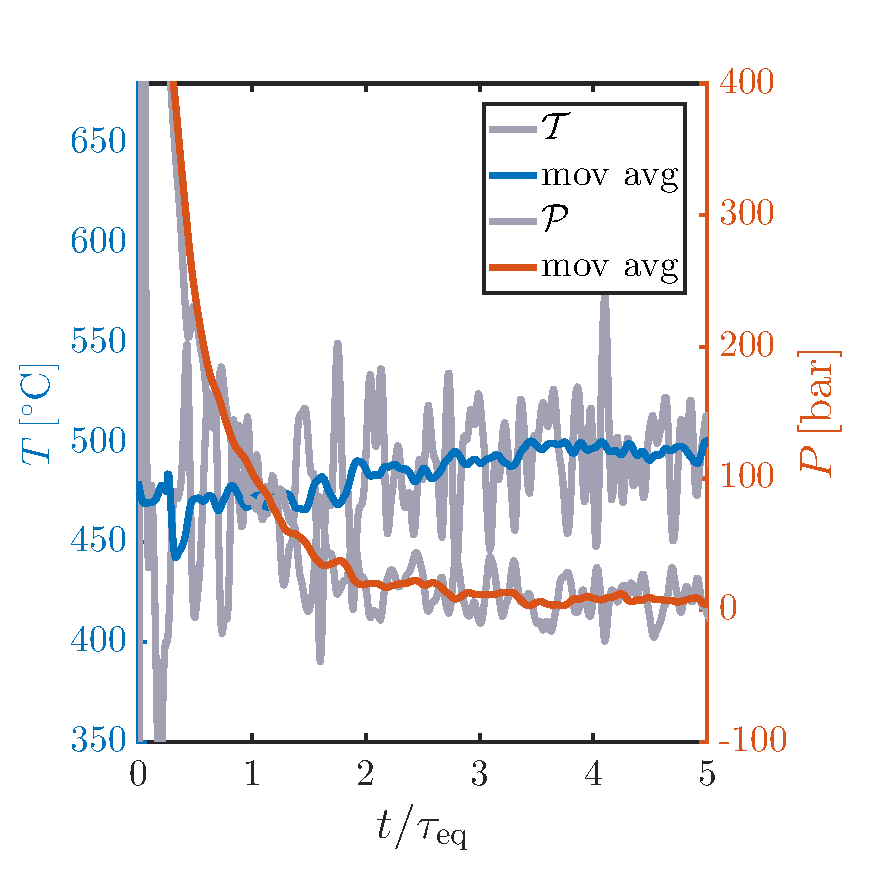
\includegraphics[width=0.48\textwidth]{../figures/TP-eq-500} 
    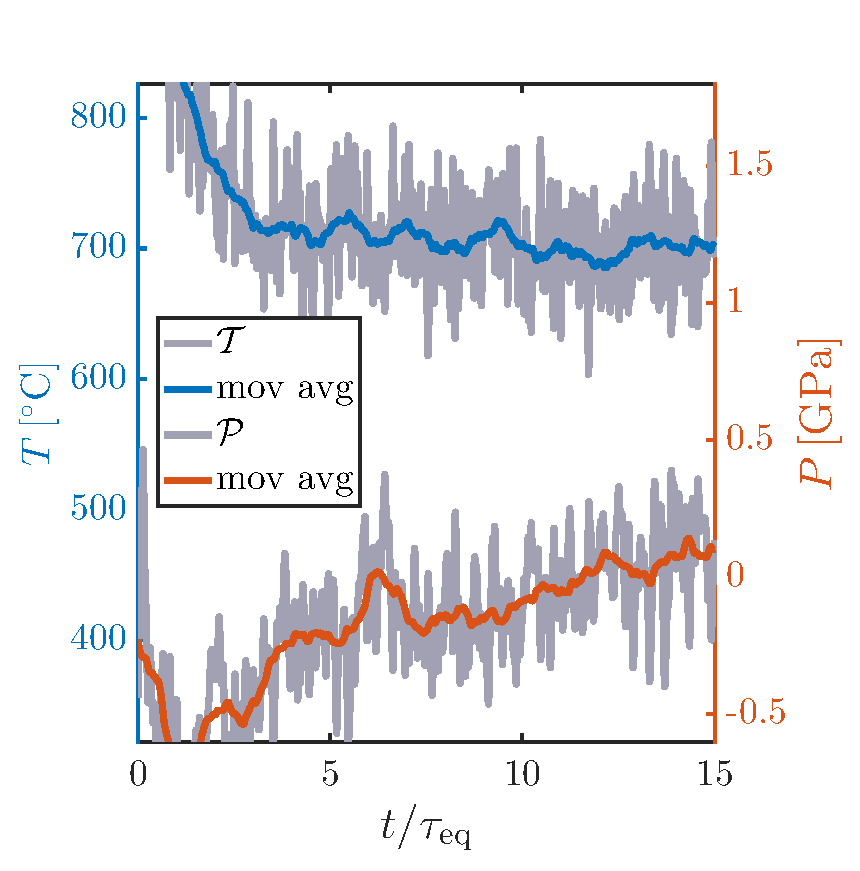
\includegraphics[width=0.48\textwidth]{../figures/TP-eq-700} 
  \caption{The instantaneous values of $\mathcal{T}$ and $\mathcal{P}$ overlayed with with a moving average using 100 time steps, which corresponds to $\Delta t = \tau_P/2$. Left panel: $T=\unit[500]{^\circ C}$,  right panel: $T=\unit[500]{^\circ C}$.}
  \label{fig:eq}
\end{center}
\end{figure}


The equilibrium values of the lattice parameter were found to be 
\begin{align}
a_0 &\approx \unit[4.10]{\AA}, \quad T=\unit[500]{^\circ C}, \\
a_0 &\approx \unit[4.29]{\AA}, \quad T=\unit[700]{^\circ C} .
\end{align} 

These value are larger than the zero-temperature constants, and it is reasonable that the higher $\unit[700]{^\circ C}$ case corresponds to a larger lattice parameter at constant pressure. 

\section*{Tasks 3-5: particle trajectories}
Starting with the temperature- and pressure equilibrated systems from the previous section, we study the particle trajectories for both systems. Here, we decrease the timestep to   $dt       = \unit[5\cdot 10^{-4}]{ps}$ and the simulation length to $t_{\rm end} = \unit[5]{ps}$ to get better statistics. This was mostly motivated by increasing the resolution in tasks 6-7. 

First, we note that the cumulative averages of the instantaneous temperatures and pressures stayed close to their inital values. This is shown in figure~\ref{fig:prod}.

\begin{figure}[!ht]
\begin{center}
  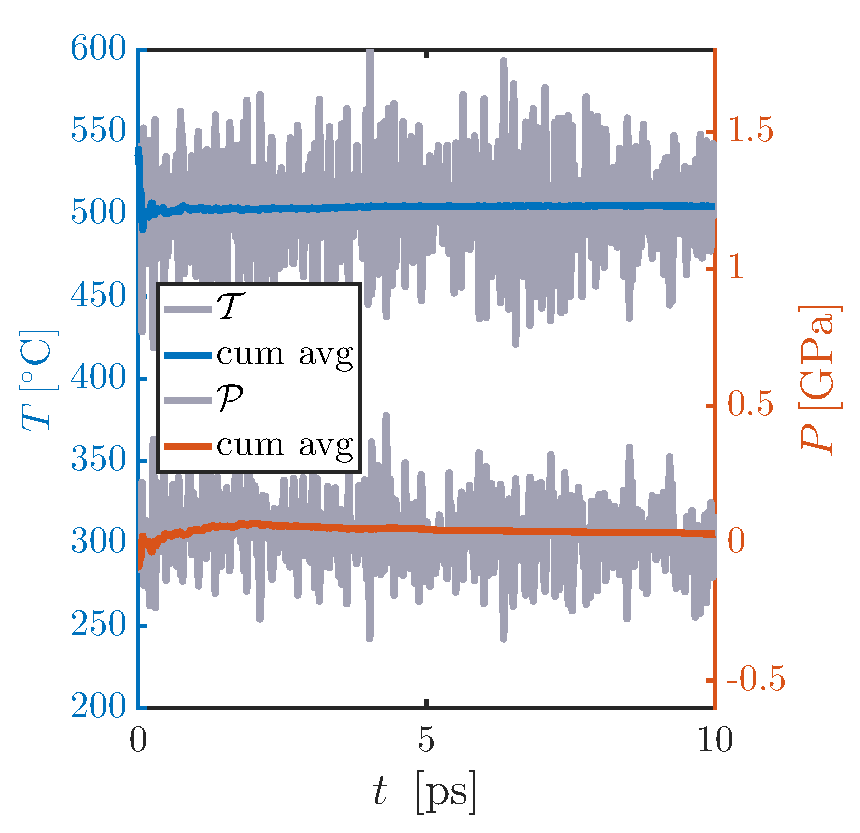
\includegraphics[width=0.48\textwidth]{../figures/TP-prod-500} 
    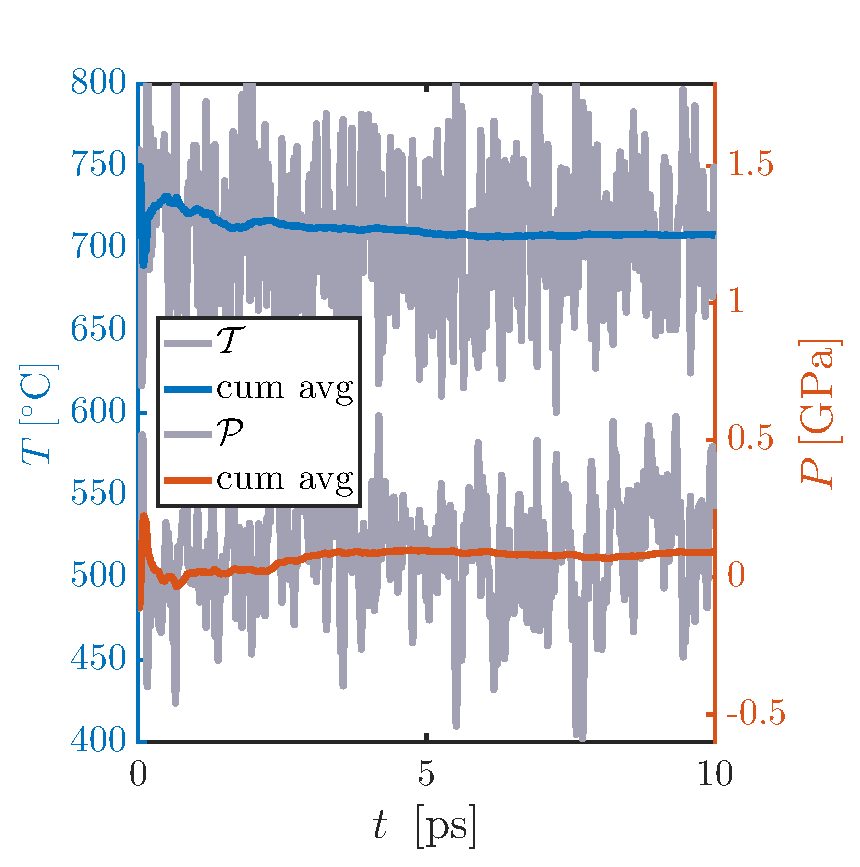
\includegraphics[width=0.48\textwidth]{../figures/TP-prod-700} 
  \caption{The instantaneous values, and the cumulative averages, of the temperature and the pressure in the production runs. Left panel: $T=\unit[500]{^\circ C}$,  right panel: $T=\unit[500]{^\circ C}$}
  \label{fig:prod}
\end{center}
\end{figure}
%%%%%%%%%%%%%%%%%%%%%%%%%%%%%%%%%%%%%%%%%%%%%%%%%%%%%

\section*{Task 5}
Equation (82) in MD lecture notes:


\begin{align}
\Delta_{\rm MSD}(t) &= \lim_{T \rightarrow \infty} \frac{1}{T} \int_0^{T} d t' \frac{1}{N_{\rm atoms}} \sum_{i=0}^{N_{\rm atoms}-1} \left[{\bf r}_i(t+t') - {\bf r}_i(t') \right]^2 \\ &\Rightarrow \nonumber
\\
\Delta_{\rm MSD}(t_k) &\approx
\frac{1}{N_T -k}\frac{1}{N_{\rm atoms}} \sum_{j=0}^{N_T-k-1} \sum_{i=0}^{N_{\rm atoms}-1} \left[{\bf r}_i(t_{k+j}) - {\bf r}_i(t_j) \right]^2 
\end{align}

To determine M, we used mean of ... for t $>$ ... 


\section*{Task 7}

% \subsection*{Sort of proof}
% Discrete auto-correlation function
% \begin{equation}
% \varPhi_j = \frac{1}{N}\sum_{i=0}^{N-1} v_{i+j}v_{i}
% \end{equation}

% Discrete Fourier transform,
% \begin{equation}
% \hat{f}_k = \sum_{i=0}^{N-1} f_i \exp(\ii 2\pi \frac{ik}{N}),
% \end{equation}
% We can define a discrete power spectrum as
% \begin{equation}
% \begin{aligned}
% \hat{P}_k =& \frac{1}{N} \abs{\hat{v}_k}^2
% =\frac{1}{N} \hat{v}_k\bar{\hat{v}}_k\\
% =&\frac{1}{N} \sum_{i=0}^{N-1} v_i\exp(\ii 2\pi \frac{ik}{N})
% \sum_{i'=0}^{N-1} v_{i'}\exp(-\ii 2\pi \frac{i'k}{N})
% \end{aligned}
% \end{equation}
% We can now do a relabeling of the index $i=i'+j$, and use periodic
% indices $v_{i+N}=v_{i}$
% \begin{equation}
% \begin{aligned}
% \hat{P}_k =& \frac{1}{N} \abs{\hat{v}_k}^2
% =\frac{1}{N} \hat{v}_k\bar{\hat{v}}_k\\
% =&\frac{1}{N} \sum_{i'=0}^{N-1}\sum_{j=-i'}^{N-1-i'} v_{j+i'}v_{i'}
% \exp(\ii 2\pi \frac{jk}{N}).
% \end{aligned}
% \end{equation}
% However, since the sum over $j$ reaches all indices in the periodic
% index domain, we can change the summation to going from $j=0$ to
% $N-1$, and then also swap the order of summation, which gives
% \begin{equation}
% \hat{P}_k =\sum_{j=0}^{N-1} \exp(\ii 2\pi \frac{jk}{N}).
% \frac{1}{N}\sum_{i'=0}^{N-1} v_{j+i'}v_{i'}.
% \end{equation}
% It is now clear that this power spectrum is the discrete Fourier
% transform of the discrete auto-correlation function,
% \begin{equation}\label{eq7:Wiener-Khinthchine}
% \hat{P}_k =\sum_{j=0}^{N-1} \varPhi_j \exp(\ii 2\pi \frac{jk}{N}).
% \end{equation}
% In reality, $v_i$ is not periodic, however we might still use the
% periodic indices for notational convenience.

\subsection*{What we did}

We calculated the discrete auto-correlation function similarly to the
MSD, 
\begin{equation}
\varPhi_j = \frac{1}{N-j}\sum_{i=0}^{N-j-1} \ev{v_{i+j}v_{i}},
\end{equation}
where $j=0,1,\ldots,N-1$ and the average is taken over all atoms.
We then preceded to numerically approximate the integral
\begin{equation}
\hat{\varPhi}(f) = 2\int_0^{\infty}\dd{t}\,
\varPhi(t) \cos(2\pi ft)
\approx 2\int_0^{T_{\rm s}}\dd{t}\,\varPhi(t) \cos(2\pi ft)
\end{equation}
using a trapeziodal method in \textsc{Matlab}, with a frequency range
$f=0$ to $f=1/(2\Delta{t})=f_{\rm Nyqvist}$, and frequency steps
$\Delta{f}=1/T_{\rm s}$, where $T_{\rm s}$ is a time at about half the
simulation end time. This is to avoid including noisy data in
$\varPhi(t)$ at later times, where the statistics are poor.

We then calculated the powerspectrum according to
\begin{equation}
\begin{aligned}
\hat{P}(\omega) =& \lim_{T\to\infty}\frac{1}{T}
\ev{\abs{\int_0^{T}\dd{t}\,v(t)\ee^{\ii\omega t}}^2}\\
\approx& \frac{1}{T}
\ev{\abs{\int_0^{T}\dd{t}\,v(t)\ee^{\ii\omega t}}^2}\\
\Longrightarrow\quad
\hat{P}_k=& \frac{1}{T}
\ev{\abs{\frac{T}{N} \sum_{i=0}^{N-1} v_i\exp(\ii2\pi\frac{ik}{N})}^2}
=\frac{T}{N} \ev{\abs{\hat{\vb*v}_k}^2}
\end{aligned}
\end{equation}
where the averages is taken over all atoms, and
\begin{equation}
\hat{\vb*v}_k = \sqrt{N}\sum_{i=0}^{N-1} \vb*v_i \exp(\ii2\pi\frac{ik}{N})
\end{equation}
is the discrete Fourier transform of $v_i$.

When we compare $\hat{\varPhi}_k$ and $\hat{P}_k$ in Figure~\ref{...},
we find that they are very similar, as, indeed, they should be
acording to the Wiener-Khinthchine theorem.







\section*{Concluding discussion}

!!!!!!!!!!!!!!!!!!!!!!!!!1

\newpage

\appendix

\section{Source Code}

Include all source code here in the appendix. Keep the code formatting clean,
use indentation, and comment your code to make it easy to understand. Also,
break lines that are too long. (Keep them under 80 characters!)

%\subsection{Calculating pi using matlab: \texttt{pi.m}}
%\lstinputlisting[language=matlab,numbers=left]{template_files/pi.m}

%\subsection{Calculating pi using python: \texttt{pi.py}}
%\lstinputlisting[language=python,numbers=left]{template_files/pi.py}


% \subsection{Main program task 1: \texttt{main\_T1.c}}
% \lstinputlisting[language=c,numbers=left]{../code/main_T1.c}

% \subsection{Main program  Task 2: \texttt{main\_T2.c}}
% \lstinputlisting[language=c,numbers=left]{../code/main_T2.c}

% \subsection{Temperature and pressure equilibration for tasks 3-7 : \texttt{main\_T3.c}}
% \lstinputlisting[language=c,numbers=left]{../code/main_T3.c}

% \subsection{Production runs for tasks 3-7 : \texttt{main\_Prod.c}}
% \lstinputlisting[language=c,numbers=left]{../code/main_Prod.c}

% \subsection{Production runs for tasks 3-7 : \texttt{main\_Prod.c}}
% \lstinputlisting[language=c,numbers=left]{../code/main_Prod.c}


% \subsection{Misc functions : \texttt{funcs.c}}
% \lstinputlisting[language=c,numbers=left]{../code/funcs.c}

% \section{Auxiliary }
% \subsection{Makefile}
% \lstinputlisting[language=bash,numbers=left]{../code/Makefile}

% \section{Matlab scripts}
% \subsection{Analysis scripts for tasks 3-7: \texttt{Al\_energies.m}}
% \lstinputlisting[language=matlab,numbers=left]{../m_scripts/H1_analysis.m}

% \subsection{Improve figure appearance: \texttt{ImproveFigureCompPhys.m}}
% \lstinputlisting[language=matlab,numbers=left]{../m_scripts/ImproveFigureCompPhys.m}

% \subsection{Change size of figures: \texttt{setFigureSize.m}}
% \lstinputlisting[language=matlab,numbers=left]{../m_scripts/setFigureSize.m}


\end{document}

%%% Local Variables:
%%% mode: latex
%%% TeX-master: t
%%% End:

%  LocalWords:  MSD
